% coding:utf-8

\section{Digitally-Controlled Oscillator}

\subsection{Übersicht}
\begin{frame}
    \frametitle{}
    \framesubtitle{}
      \begin{figure}
        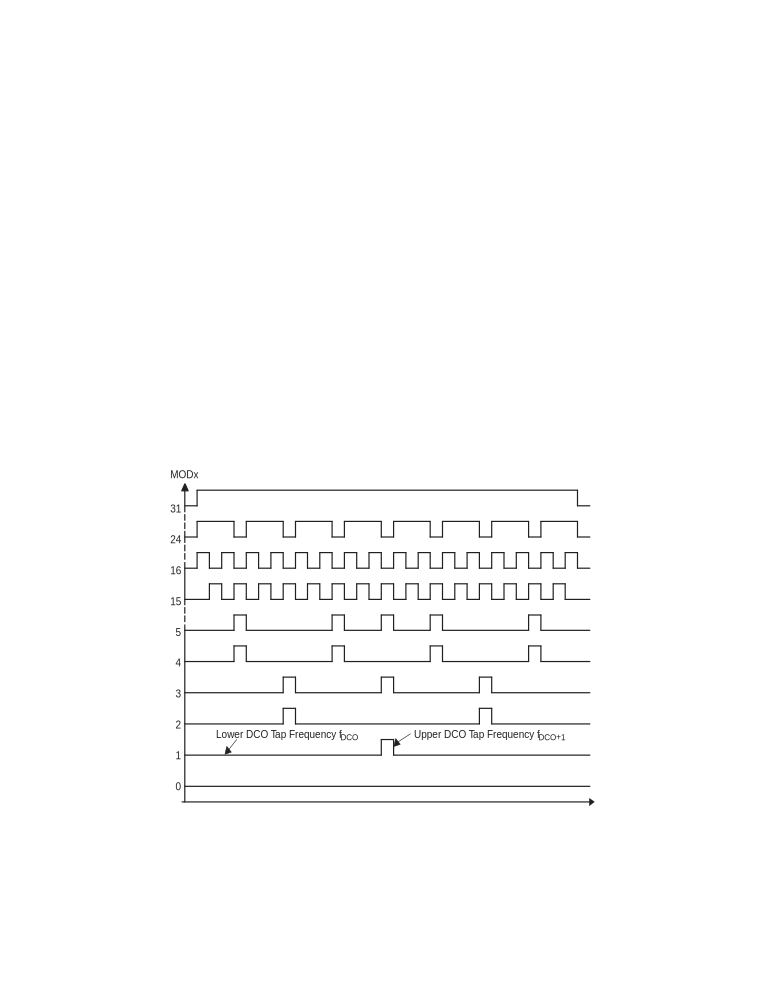
\includegraphics[width=0.7\columnwidth]{fig/ti_fg_dco_mod.pdf}
        \caption{Funktionsweise Modulation}
      \end{figure}
\end{frame}

\begin{frame}
  \begin{tikztimingtable}
    \mbox{\uncover<1->{MOD =  0}} & <1->33L<*>\\
    \mbox{\uncover<2->{MOD =  1}} & <2->16LH16L<*>\\
    \mbox{\uncover<3->{MOD = 31}} & <3->L31HL<*>\\
    \mbox{\uncover<4->{MOD = 24}} & <4->L3HL3HL3HL3HL3HL3HL3HL3HL<*>\\
  \end{tikztimingtable}
\end{frame}